\documentclass{bioinfo}
\copyrightyear{2015} \pubyear{2015}

\access{Advance Access Publication Date: Day Month Year}
\appnotes{Manuscript Category}

\begin{document}
\firstpage{1}

\subtitle{Subject Section}

\title[short Title]{Prediction of amyloidogenicity based on the n-gram analysis}
\author[Sample \textit{et~al}.]{Micha\l{} Burdukiewicz$^{\text{\sfb 1,*}}$, Piotr Sobczyk\,$^{\text{\sfb 2}}$, Pawe\l{} Mackiewicz$^{\text{\sfb 1}}$ and Ma\l{}gorzata Kotulska\,$^{\text{\sfb 3,}*}$}
\address{$^{\text{\sf 1}}$University of Wroc\l{}aw, Department of Genomics,
$^{\text{\sf 2}}$Wroc\l{}aw University of Technology, Department of Mathematics and 
$^{\text{\sf 3}}$Wroc\l{}aw University of Technology, Department of Biomedical Engineering, Faculty of Fundamental Problems of Technology
}


\corresp{$^\ast$To whom correspondence should be addressed.}

\history{Received on XXXXX; revised on XXXXX; accepted on XXXXX}

\editor{Associate Editor: XXXXXXX}

\abstract{\textbf{Motivation:} Text Text Text Text Text Text Text Text Text Text Text Text Text
Text Text Text Text Text Text Text Text Text Text Text Text Text Text Text Text Text Text Text
Text Text Text Text Text Text Text Text Text Text Text Text Text Text Text Text Text Text Text
Text Text Text Text Text Text
Text Text Text Text Text.\\
\textbf{Results:} Text  Text Text Text Text Text Text Text Text Text  Text Text Text Text Text
Text Text Text Text Text Text Text Text Text Text Text Text Text  Text Text Text Text Text Text\\
\textbf{Availability:} Text  Text Text Text Text Text Text Text Text Text  Text Text Text Text
Text Text Text Text Text Text Text Text Text Text Text Text Text Text  Text\\
\textbf{Contact:} \href{name@bio.com}{name@bio.com}\\
\textbf{Supplementary information:} Supplementary data are available at \textit{Bioinformatics}
online.}

\maketitle

\section{Introduction}

Text Text Text Text Text Text  Text Text Text Text Text Text Text
Text Text  Text Text Text Text Text Text. Figure~\ref{fig:01}
shows that the above method  Text Text Text Text  Text Text Text
Text Text Text  Text Text.  \citep{Bag01} wants to know about
{\ldots}{\ldots} text follows.
\begin{equation}
\sum \text{\it x}+ \text{\it y} =\text{\it Z}\label{eq:01}\vspace*{-10pt}
\end{equation}

%\enlargethispage{12pt}

\section{Approach}

Equation~(\ref{eq:01}) Text Text Text Text Text Text  Text Text
Text Text Text Text Text Text Text Text Text Text Text Text Text.
Figure~2\vphantom{\ref{fig:02}} shows that the above method  Text
Text Text Text  Text Text Text Text Text Text  Text Text.
\citealp{Boffelli03} might want to know about text text text text
.....


\begin{methods}
\section{Methods}

\subsection{Data set}

The data used in the study was extracted from AmyLoad data base~\citep{wozniak_amyload:_2015}. Aside from eight sequences shorter than five residues that were removed from the final data set, we obtained 418 amyloidogenic sequences and 1039 non-amyloidogenic sequences (1457 peptides in total).

Sequences shorter than 6 amino acids and longer than 25 amino acids were removed from data set. The former were too short to be processed in the devised analysis framework and the latter were too diversified and rare, preventing the proper analysis.

The final data set contains 397 amyloidogenic and 1033 non-amyloidogenic sequences (1430 peptides in total).

\subsection{Encodings of amino acids}

The amyloidogenicity of given peptide may not depend on the exact sequence of amino acids, but on its more general properties. To verify this hypothesis, we created 18 537 reduced amino acid alphabets with different lengths (from three to six letters).

We created the reduced alphabet of amino acids using Ward's clusterization on the selected physicochemical properties from AAIndex database~\citep{kawashima_aaindex:_2008}. We handpicked several measures belonging to more general categories important in process of amyloidogenicity as size, hydrophobicity, solvent surface area, frequency in $\beta$-sheets and contactivity. As the rule of thumb, we limited ourselves to properties introduced after 1980 when, thanks to the technological advancements, the measurements were more accurate.

\begin{table}[ht]
\centering
\begin{tabular}{ll}
  \hline
Category & Property \\ 
  \hline
  Contactivity & Average flexibility indices \citep{bhaskaran_positional_1988} \\ 
  Contactivity & 14 A contact number \citep{nishikawa_radial_1986} \\ 
  Contactivity & Accessible surface area \citep{radzicka_comparing_1988} \\ 
    Contactivity & Buriability \citep{zhou_quantifying_2004} \\ 
  Contactivity & Values of Wc in proteins from class Beta, cutoff 12 A, separation 5 \citep{wozniak_characteristics_2014} \\ 
  Contactivity & Values of Wc in proteins from class Beta, cutoff 12 A, separation 15 \citep{wozniak_characteristics_2014} \\ 
  $\beta$-frequency & Average relative probability of inner beta-sheet \citep{kanehisa_local_1980} \\ 
  $\beta$-frequency & Relative frequency in beta-sheet \citep{prabhakaran_distribution_1990} \\ 
  $\beta$-frequency & Thermodynamic beta sheet propensity \citep{kim_thermodynamic_1993} \\ 
  Hydrophobicity & Hydrophobicity index \citep{argos_structural_1982} \\ 
  Hydrophobicity & Optimal matching hydrophobicity \citep{sweet_correlation_1983} \\ 
  Hydrophobicity & Hydrophobicity-related index \citep{kidera_statistical_1985} \\ 
  Hydrophobicity & Scaled side chain hydrophobicity values \citep{black_development_1991} \\ 
  Polarity & Polarizability parameter \citep{charton_structural_1982} \\ 
  Polarity & Mean polarity \citep{radzicka_comparing_1988} \\ 
  Size & Average volumes of residues \citep{pontius_deviations_1996} \\ 
  Stability & Side-chain contribution to protein stability (kJ/mol) \citep{takano_new_2001} \\ 
   \hline
\end{tabular}
\caption{Physicochemical properties used during creation of reduced amino acid alphabets.} 
\end{table}

Since highly correlated or, contrarily, uncorrelated measures create very similar encodings, we further reduced the number of properties to 17 by selecting measures with the Pearson's correlation coefficient for normalized values larger than 0.95 or smaller than 0.05.

\subsection{Traning of learners}


\begin{figure*}[!tpb]%figure1
\centerline{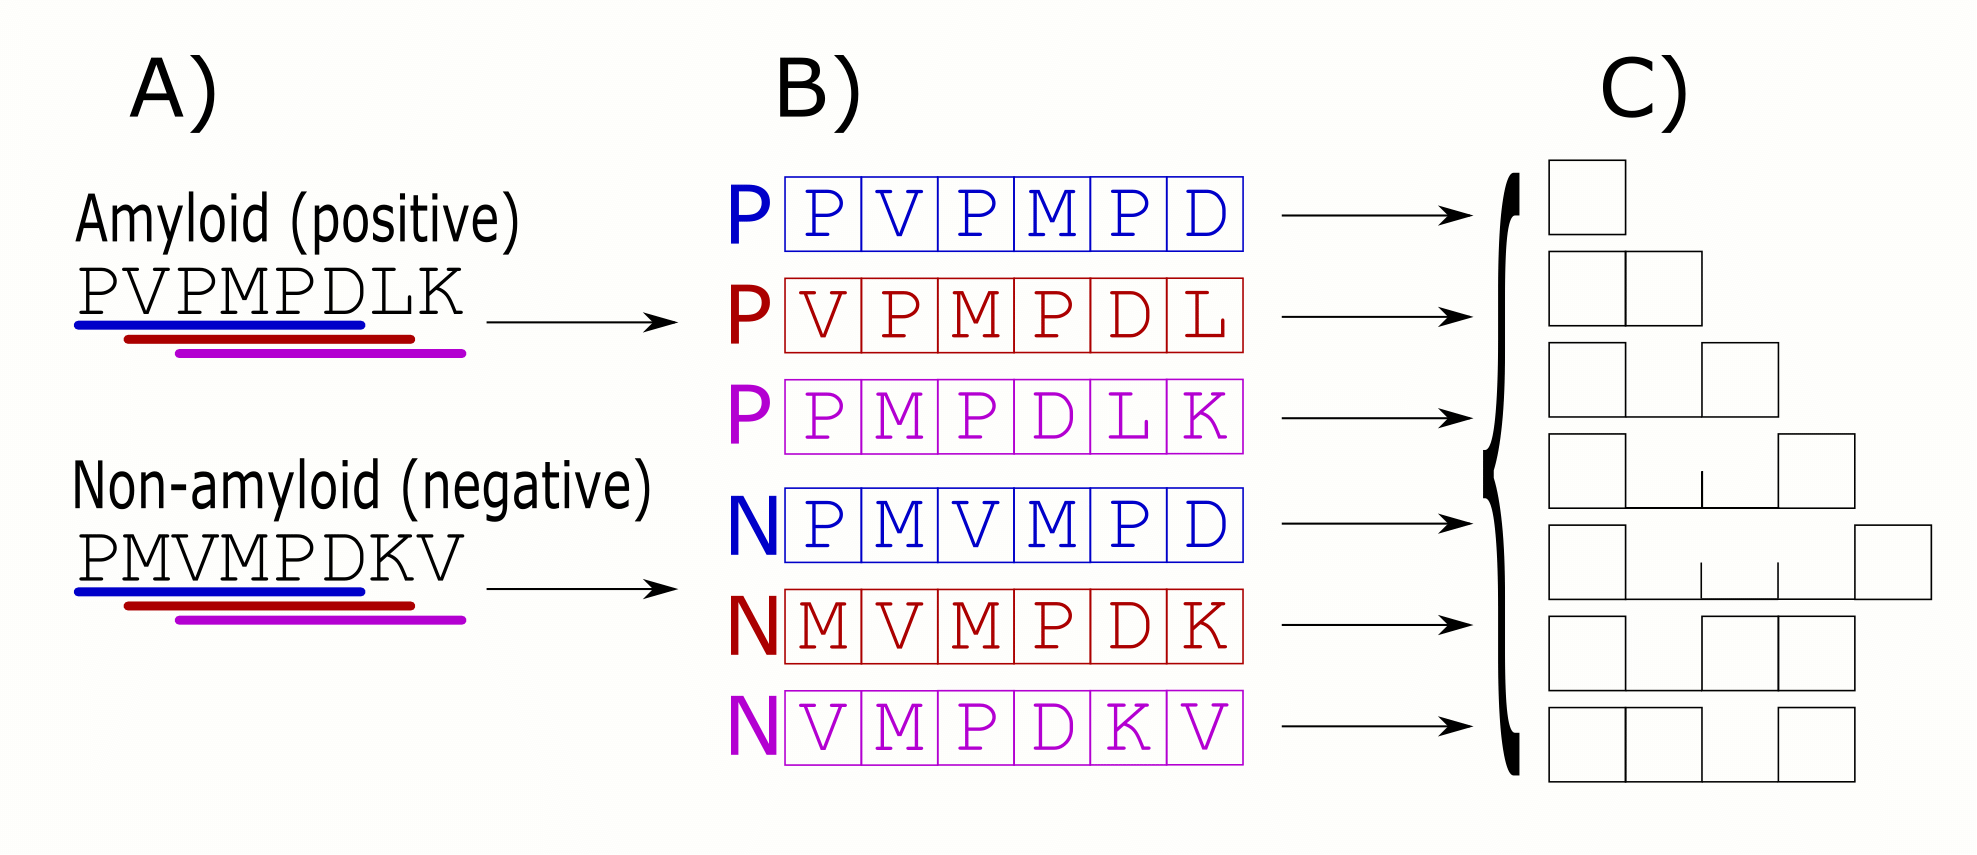
\includegraphics[width=\textwidth]{figures/ngram_scheme.png}}
\caption{Caption, caption.}\label{fig:01}
\end{figure*}

In addition to the reduced amino acid alphabets created through the clusterization of physicochemical properties, we also examined two reduced alphabets from the literature and raw amino acid sequences.  

Assuming that in longer amyloids only the short part of the sequence is responsible for amyloidogenicity, 
we restricted the maximum length of peptides in training data set to fifteen amino acids to easy the extraction of probable hot-spots. During the training phase, we extracted overlapping hexamers from each sequence. Each hexamer was tagged with the same etiquette (amyloid/nonamyloid) as the original peptide. For example, the sequence of length 6 residues yields only one hexamer and the sequence of 8 residues yields 3 hexamers. 

The inquire the exact length of amyloidogenicity signal, we trained nine classifiers for each encoding on the sequences of different length. We considered sequences of length 6, shorter of equal to 10 residues and shorter or equal to 15 residues. We specified separately length of peptides for negative and positive training set, obtaining in total nine classifiers per each encoding.

\subsection{Cross-validation}

The cross-validation was repeated five times for each combination of the encoding as well as the length of sequences in positive data set and negative data set.

Since we are interested if our classiffiers are able to use decision rules extracted from sequences of given length to correctly classify longer or shorter sequences, we calculate performance measures separately for four ranges of lengths of sequences:  
\begin{itemize}
\item 6;  
\item 7-10;   
\item 11-15;   
\item 16-25.  
\end{itemize}
The number of sequences from the given length range was roughly comparable between folds of cross-validation.


\section{Discussion}

Text Text Text Text Text Text  Text Text Text Text Text Text Text
Text Text  Text Text Text Text Text Text.
Figure~2\vphantom{\ref{fig:02}} shows that the above method  Text
Text Text Text  Text Text Text Text Text Text  Text Text.
\citealp{Boffelli03} might want to know about  text text text text
Text Text Text Text Text Text  Text Text Text Text Text Text Text
Text Text  Text Text Text Text Text Text.
Figure~2\vphantom{\ref{fig:02}} shows that the above method  Text
Text Text Text  Text Text Text Text Text Text  Text Text.
\citealp{Boffelli03} might want to know about  text text text text
Text Text Text Text Text Text Text Text Text Text.




Table~\ref{Tab:01} shows that Text Text Text Text Text  Text Text
Text Text Text Text. Figure~2\vphantom{\ref{fig:02}} shows that
the above method Text Text. Text Text Text  Text Text Text Text
Text Text. Figure~2\vphantom{\ref{fig:02}} shows that the above
method Text Text. Text Text Text  Text Text Text Text Text Text.
Figure~2\vphantom{\ref{fig:02}} shows that the above method Text
Text.









%%%%%%%%%%%%%%%%%%%%%%%%%%%%%%%%%%%%%%%%%%%%%%%%%%%%%%%%%%%%%%%%%%%%%%%%%%%%%%%%%%%%%
%
%     please remove the " % " symbol from \centerline{\includegraphics{fig01.eps}}
%     as it may ignore the figures.
%
%%%%%%%%%%%%%%%%%%%%%%%%%%%%%%%%%%%%%%%%%%%%%%%%%%%%%%%%%%%%%%%%%%%%%%%%%%%%%%%%%%%%%%






\section{Conclusion}

(Table~\ref{Tab:01}) Text Text Text Text Text Text  Text Text Text
Text Text Text Text Text Text  Text Text Text Text Text Text.
Figure~2\vphantom{\ref{fig:02}} shows that the above method  Text
Text Text Text  Text Text Text Text Text Text  Text Text.
\citealp{Boffelli03} might want to know about  text text text text
Text Text Text Text Text Text  Text Text Text Text Text Text Text
Text Text  Text Text Text Text Text Text.
Figure~2\vphantom{\ref{fig:02}} shows that the above method  Text
Text Text Text  Text Text Text Text Text Text  Text Text.
\citealp{Boffelli03} might want to know about  text text text text
Text Text Text Text Text Text Text Text Text Text Text Text Text
Text Text  Text Text Text Text Text Text.
Figure~2\vphantom{\ref{fig:02}} shows that the above method  Text
Text Text Text  Text Text Text Text Text Text  Text Text.



Text Text Text Text Text Text  Text Text Text Text Text Text Text
Text Text  Text Text Text Text Text Text.
Figure~2\vphantom{\ref{fig:02}} shows that the above method  Text
Text Text Text  Text Text Text Text Text Text  Text Text.
\citealp{Boffelli03} might want to know about  text text text text

\begin{enumerate}
\item this is item, use enumerate
\item this is item, use enumerate
\item this is item, use enumerate
\end{enumerate}

Text Text Text Text Text Text Text Text Text Text Text Text Text
Text Text Text Text Text Text Text Text.
Figure~2\vphantom{\ref{fig:02}} shows\vadjust{\pagebreak} that the
above method  Text Text Text Text Text Text Text Text Text Text
Text Text.  \citealp{Boffelli03} might want to know about text
text text text Text Text Text Text Text Text  Text Text Text Text
Text Text Text Text Text Text Text Text Text Text Text.
Figure~2\vphantom{\ref{fig:02}} shows that the above method  Text
Text Text Text Text Text Text Text Text Text  Text Text.
\citealp{Boffelli03} might want to know about text text text text
Text Text Text Text Text Text  Text Text Text Text Text Text Text
Text Text Text Text Text Text Text\break Text.


Text Text Text Text Text Text  Text Text Text Text Text Text Text
Text Text  Text Text Text Text Text Text.
Figure~2\vphantom{\ref{fig:02}} shows that the above method  Text
Text Text Text\vspace*{-10pt}


\section*{Acknowledgements}

Text Text Text Text Text Text  Text Text.  \citealp{Boffelli03} might want to know about  text
text text text\vspace*{-12pt}

\section*{Funding}

The conference fee was funded by the KNOW Consortium.

\bibliographystyle{natbib}
%\bibliographystyle{achemnat}
%\bibliographystyle{plainnat}
%\bibliographystyle{abbrv}
%\bibliographystyle{bioinformatics}
%
%\bibliographystyle{plain}
%
\bibliography{amyloids}


\end{document}
